% How virtual populations get built, and what each construction hands back.
% The right-hand column is the point: the first three return one object, this
% model returns a distribution over populations.
%
%   compile:  pdflatex landscape.tex
%
\documentclass[border=10pt]{standalone}
\usepackage{lmodern}
\usepackage{amsmath}
\usepackage{amssymb}
\usepackage{tikz}
\usetikzlibrary{arrows.meta,positioning,calc}
% Shared palette for the population-model figures.
%   ink      body / structure
%   popcol   the patient cloud and anything predicted from it
%   mechcol  the simulator and species-level quantities
%   msrcol   the measurement map (readout-level: gamma, kappa)
%   datacol  reported rows
\definecolor{ink}{HTML}{3A3A3A}
\definecolor{popcol}{HTML}{3B4AA6}
\definecolor{mechcol}{HTML}{2E7D5B}
\definecolor{msrcol}{HTML}{EB811B}
\definecolor{datacol}{HTML}{8C3B4A}


\begin{document}
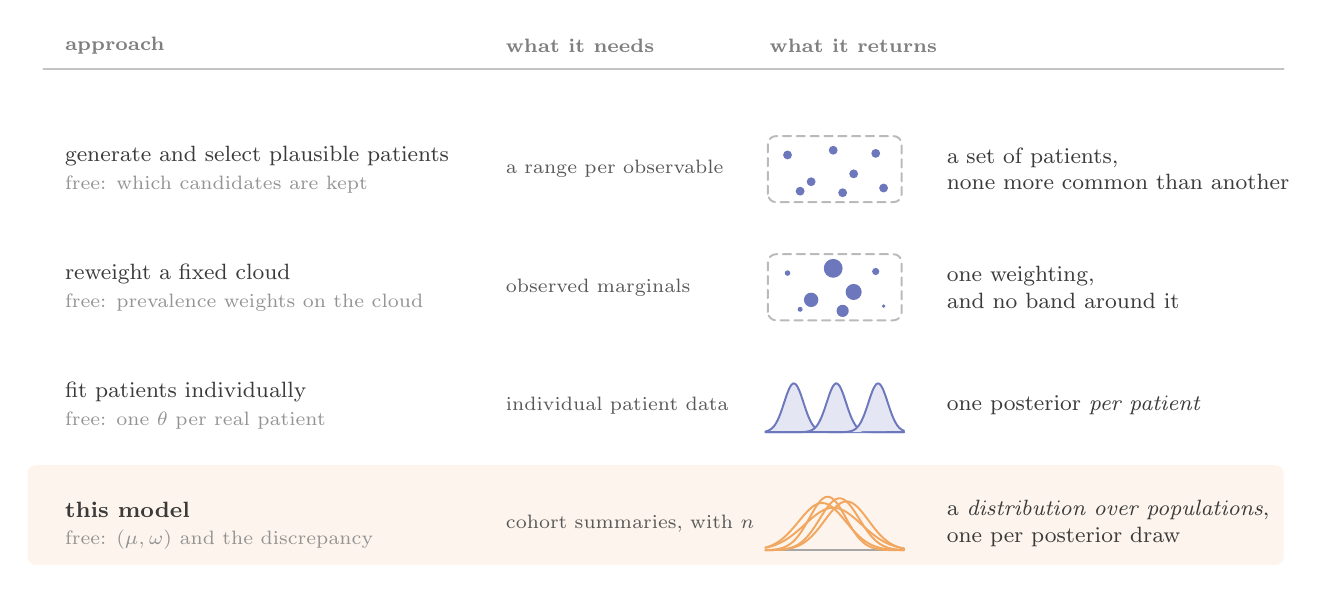
\begin{tikzpicture}[
  font=\sffamily, line cap=round, line join=round,
  hdr/.style={font=\scriptsize\bfseries, text=ink!65, anchor=west},
  nm/.style={font=\footnotesize, text=ink, anchor=west},
  fre/.style={font=\scriptsize, text=ink!55, anchor=west},
  nd/.style={font=\scriptsize, text=ink!85, anchor=west, align=left,
            text width=32mm},
  ret/.style={font=\footnotesize, text=ink, anchor=west, align=left}]

\def\xa{0}        % approach
\def\xb{5.6}      % what it needs
\def\xc{9.9}      % pictogram centre
\def\xd{11.2}     % what it returns

% ---------------------------------------------------------------- header
\node[hdr] at (\xa,1.15) {approach};
\node[hdr] at (\xb,1.15) {what it needs};
\node[hdr] at ({\xc-0.95},1.15) {what it returns};
\draw[ink!30, line width=0.7pt] (-0.15,0.85) -- (15.6,0.85);

% ---------------------------------------------------------------- row 4 highlight
\fill[msrcol!8, rounded corners=3pt] (-0.35,-5.45) rectangle (15.6,-4.18);

% ================================================================ row 1
\node[nm]  at (\xa,-0.25) {generate and select plausible patients};
\node[fre] at (\xa,-0.62) {free: which candidates are kept};
\node[nd]  at (\xb,-0.42) {a range per observable};
\begin{scope}[shift={(\xc,-0.42)}]
  \draw[ink!35, densely dashed, rounded corners=3pt, line width=0.7pt]
    (-0.85,-0.42) rectangle (0.85,0.42);
  \foreach \x/\y in {-0.60/0.18, -0.30/-0.16, -0.02/0.24, 0.24/-0.06,
                     0.52/0.20, -0.44/-0.28, 0.62/-0.24, 0.10/-0.30}
    \fill[popcol!75] (\x,\y) circle (1.6pt);
\end{scope}
\node[ret] at (\xd,-0.42) {a set of patients,\\ none more common than another};

% ================================================================ row 2
\node[nm]  at (\xa,-1.75) {reweight a fixed cloud};
\node[fre] at (\xa,-2.12) {free: prevalence weights on the cloud};
\node[nd]  at (\xb,-1.92) {observed marginals};
\begin{scope}[shift={(\xc,-1.92)}]
  \draw[ink!35, densely dashed, rounded corners=3pt, line width=0.7pt]
    (-0.85,-0.42) rectangle (0.85,0.42);
  \foreach \x/\y/\r in {-0.60/0.18/1.0, -0.30/-0.16/2.6, -0.02/0.24/3.4,
                        0.24/-0.06/2.9, 0.52/0.20/1.3, -0.44/-0.28/0.9,
                        0.62/-0.24/0.7, 0.10/-0.30/2.2}
    \fill[popcol!75] (\x,\y) circle (\r pt);
\end{scope}
\node[ret] at (\xd,-1.92) {one weighting,\\ and no band around it};

% ================================================================ row 3
\node[nm]  at (\xa,-3.25) {fit patients individually};
\node[fre] at (\xa,-3.62) {free: one $\theta$ per real patient};
\node[nd]  at (\xb,-3.42) {individual patient data};
\begin{scope}[shift={(\xc,-3.42)}]
  \draw[ink!45, line width=0.6pt] (-0.88,-0.34) -- (0.88,-0.34);
  \foreach \m in {-0.52, 0.02, 0.55}
    \draw[popcol!75, fill=popcol!14, line width=0.7pt]
      plot[domain=-0.88:0.88,samples=46,smooth]
        (\x,{-0.34+0.62*exp(-(\x-\m)*(\x-\m)/0.030)});
\end{scope}
\node[ret] at (\xd,-3.42) {one posterior \emph{per patient}};

% ================================================================ row 4
\node[nm]  at (\xa,-4.75) {\textbf{this model}};
\node[fre] at (\xa,-5.12) {free: $(\mu,\omega)$ and the discrepancy};
\node[nd]  at (\xb,-4.92) {cohort summaries, with $n$};
\begin{scope}[shift={(\xc,-4.92)}]
  \draw[ink!45, line width=0.6pt] (-0.88,-0.34) -- (0.88,-0.34);
  \foreach \m/\sd/\h in {-0.16/0.30/0.60, 0.06/0.25/0.66, -0.02/0.36/0.54,
                         0.15/0.28/0.62, -0.09/0.23/0.68}
    \draw[msrcol!70, line width=0.7pt]
      plot[domain=-0.88:0.88,samples=52,smooth]
        (\x,{-0.34+\h*exp(-(\x-\m)*(\x-\m)/(2*\sd*\sd))});
\end{scope}
\node[ret] at (\xd,-4.92) {a \emph{distribution over populations},\\ one per posterior draw};

\end{tikzpicture}
\end{document}
